% Charlotte Geiger - Manuel Lippert - Leonard Schatt
% Physikalisches Praktikum

% Teilauswertung 2

\def\weite{4cm}

\section{Umkehrintegrator}
\begin{center}
    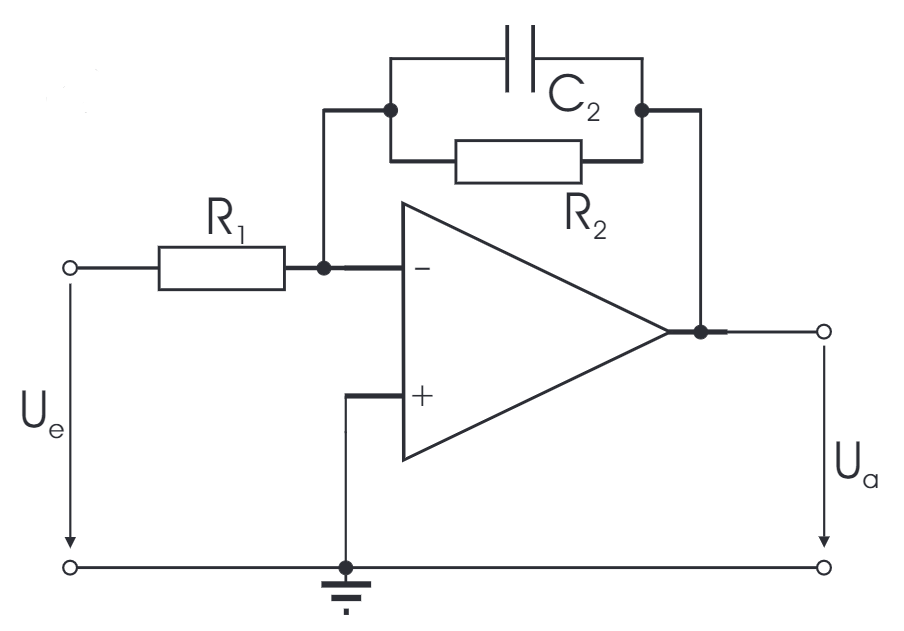
\includegraphics[scale = 0.4]{intOPV_verbessert.PNG}
    \captionof{figure}{Modifizierte Version eines Umkehrintegrators}
\end{center}
Bei der Betrachtung von Abbildung \ref{abb:int} wird deutlich, dass der Umkehrintegrator bei zunehmender Frequenz immer besser integriert und die dadurch entstehende Dreiecksspannung immer besser sichbar wird.
\begin{center}
    \begin{tabular}{c c c}
        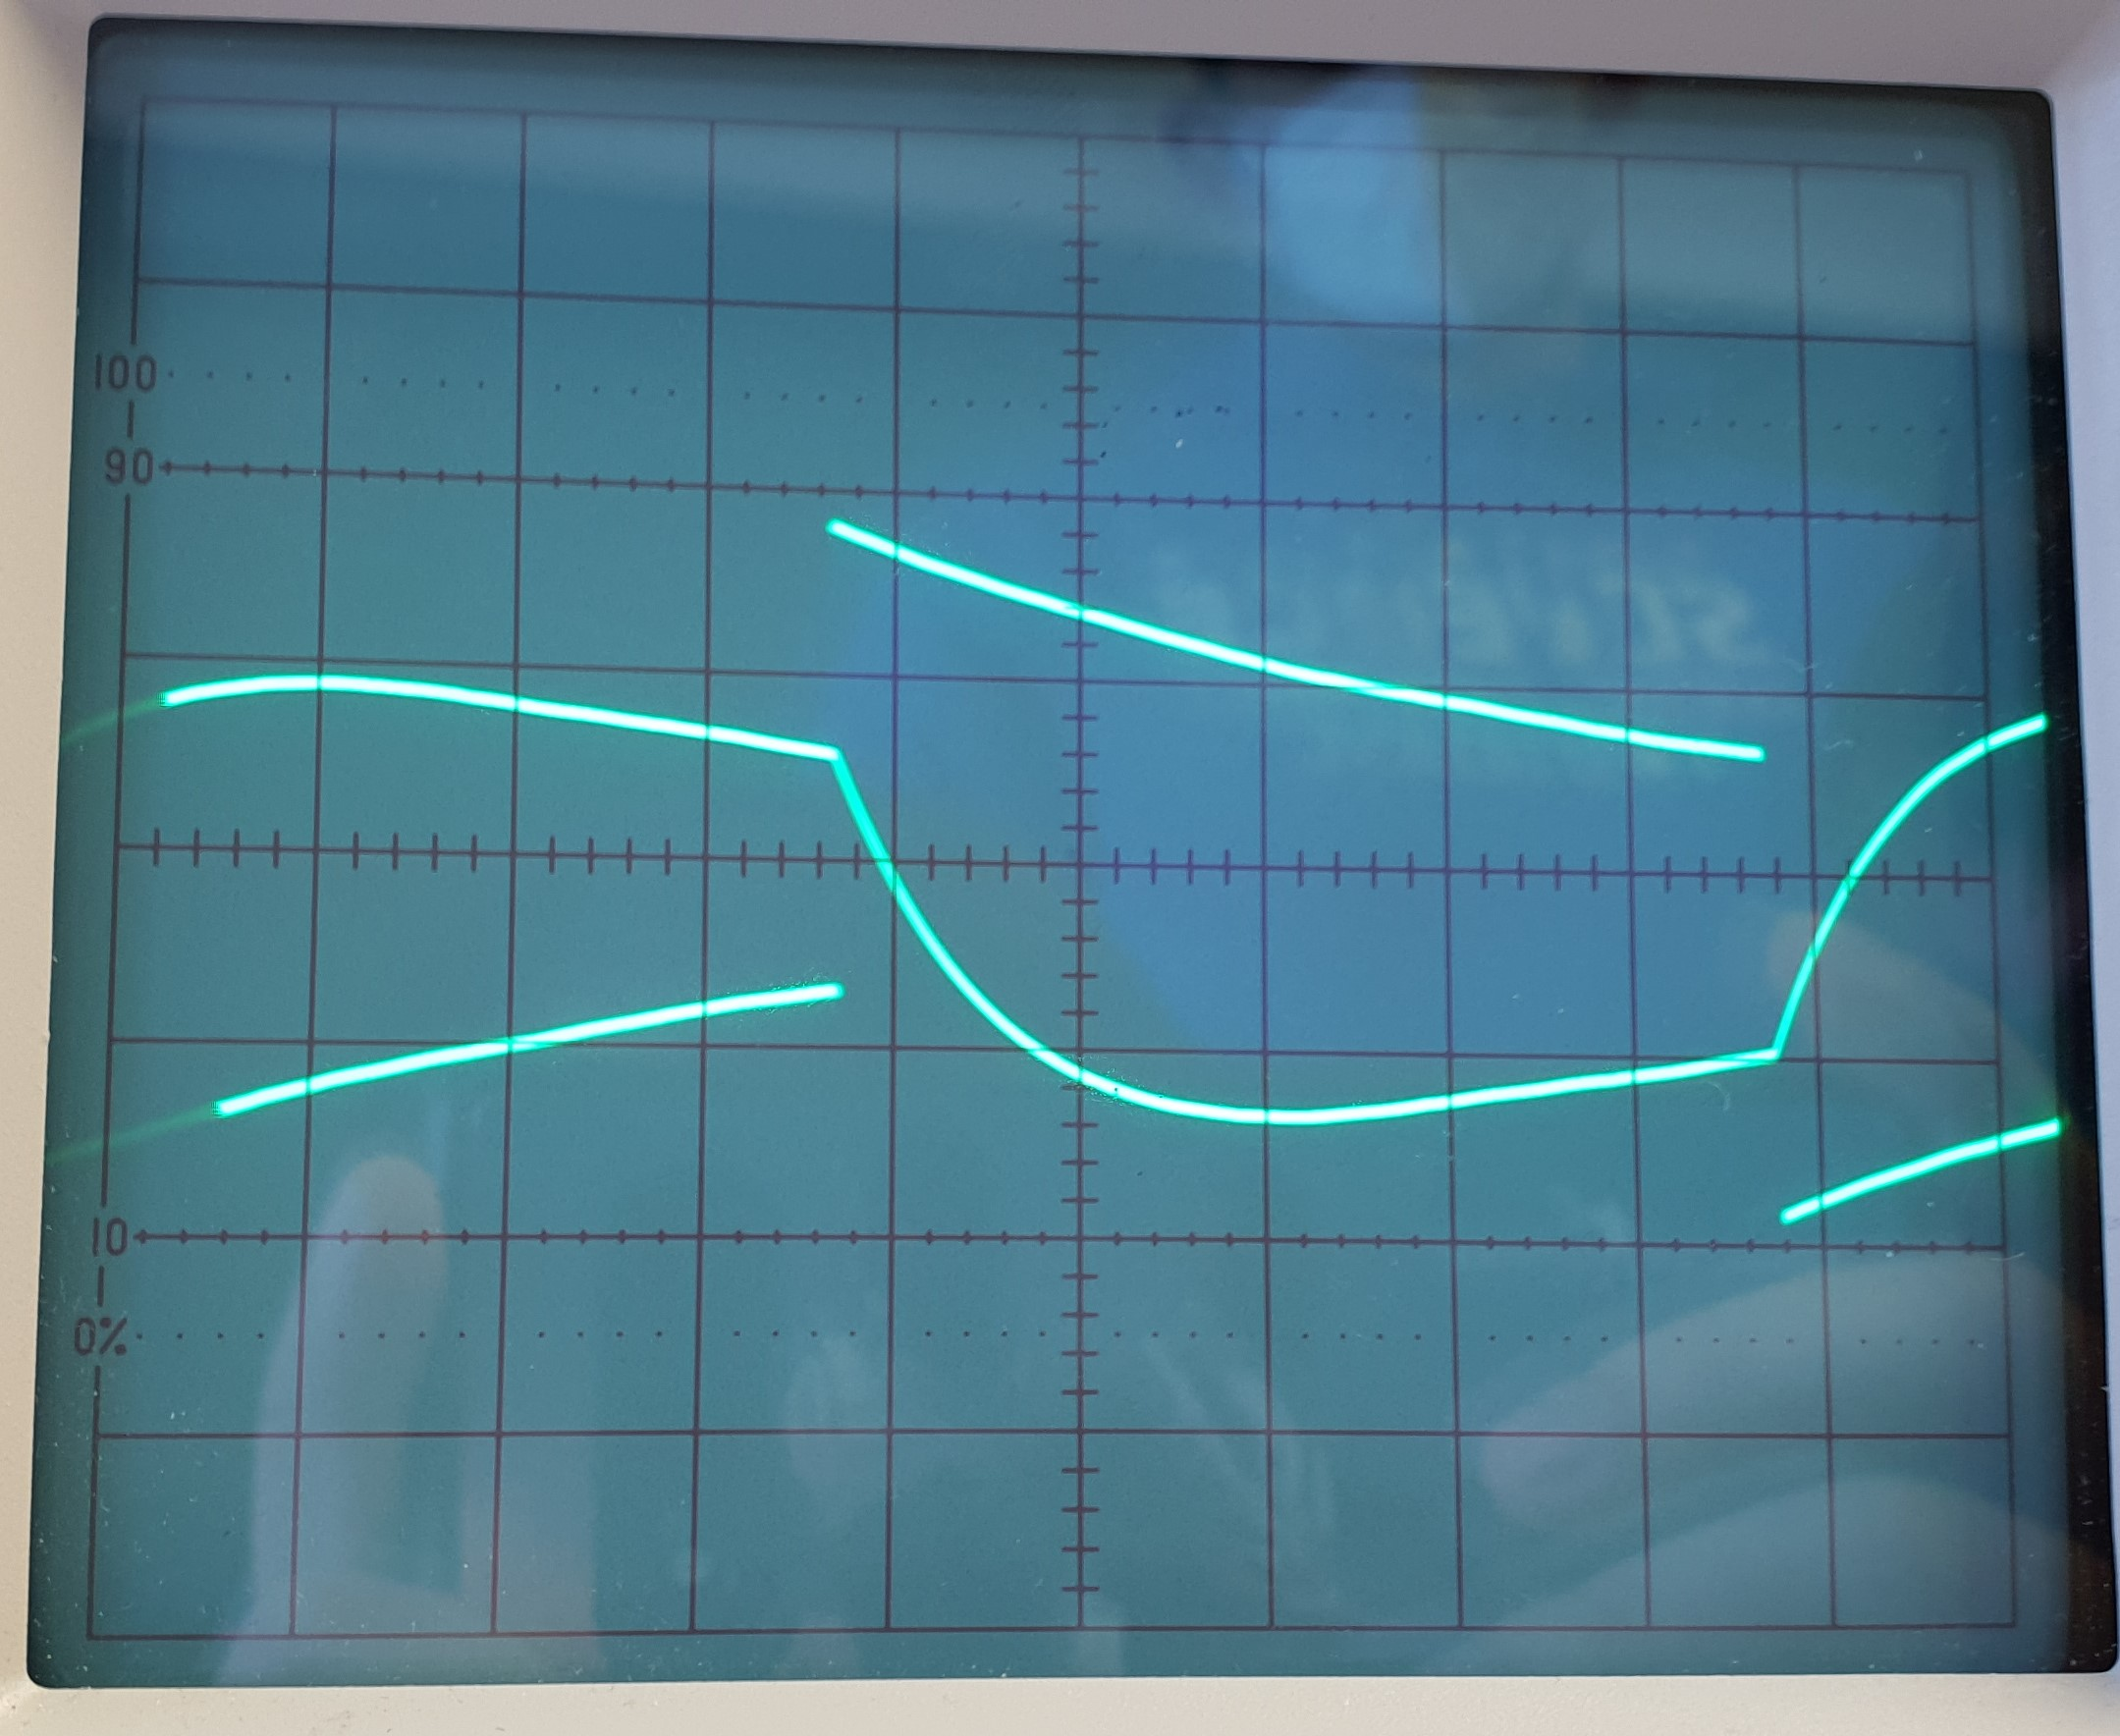
\includegraphics[width = \weite]{42-10Hz.jpg} & 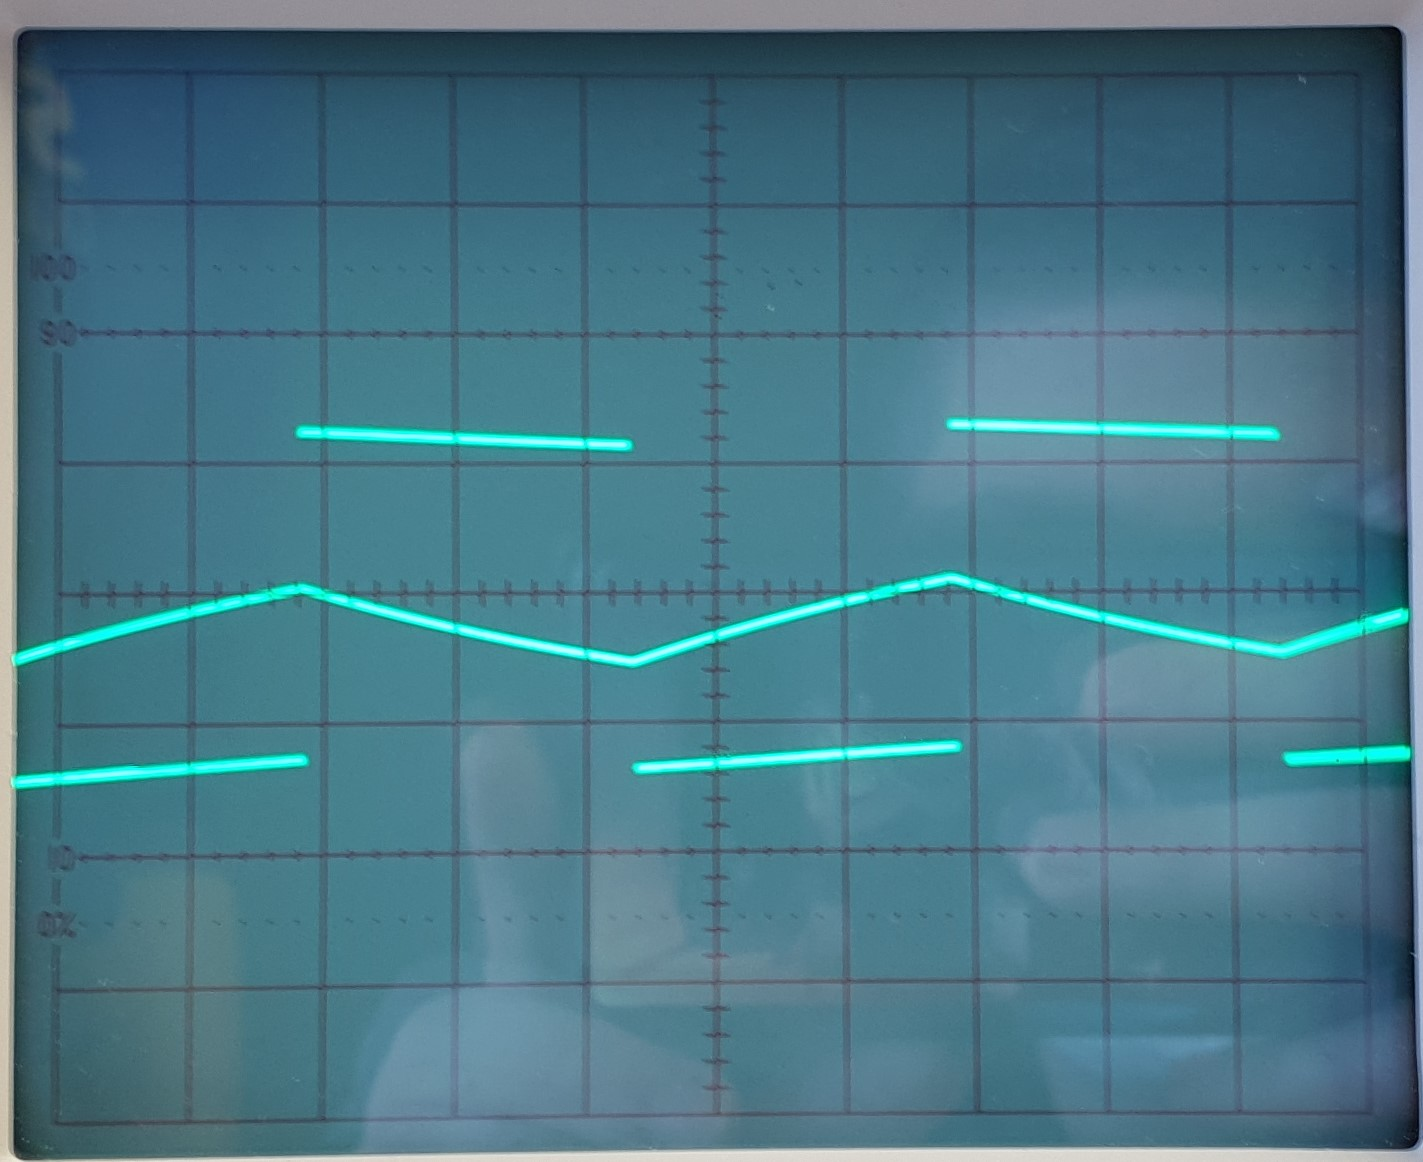
\includegraphics[width = \weite]{42-100Hz.jpg} & 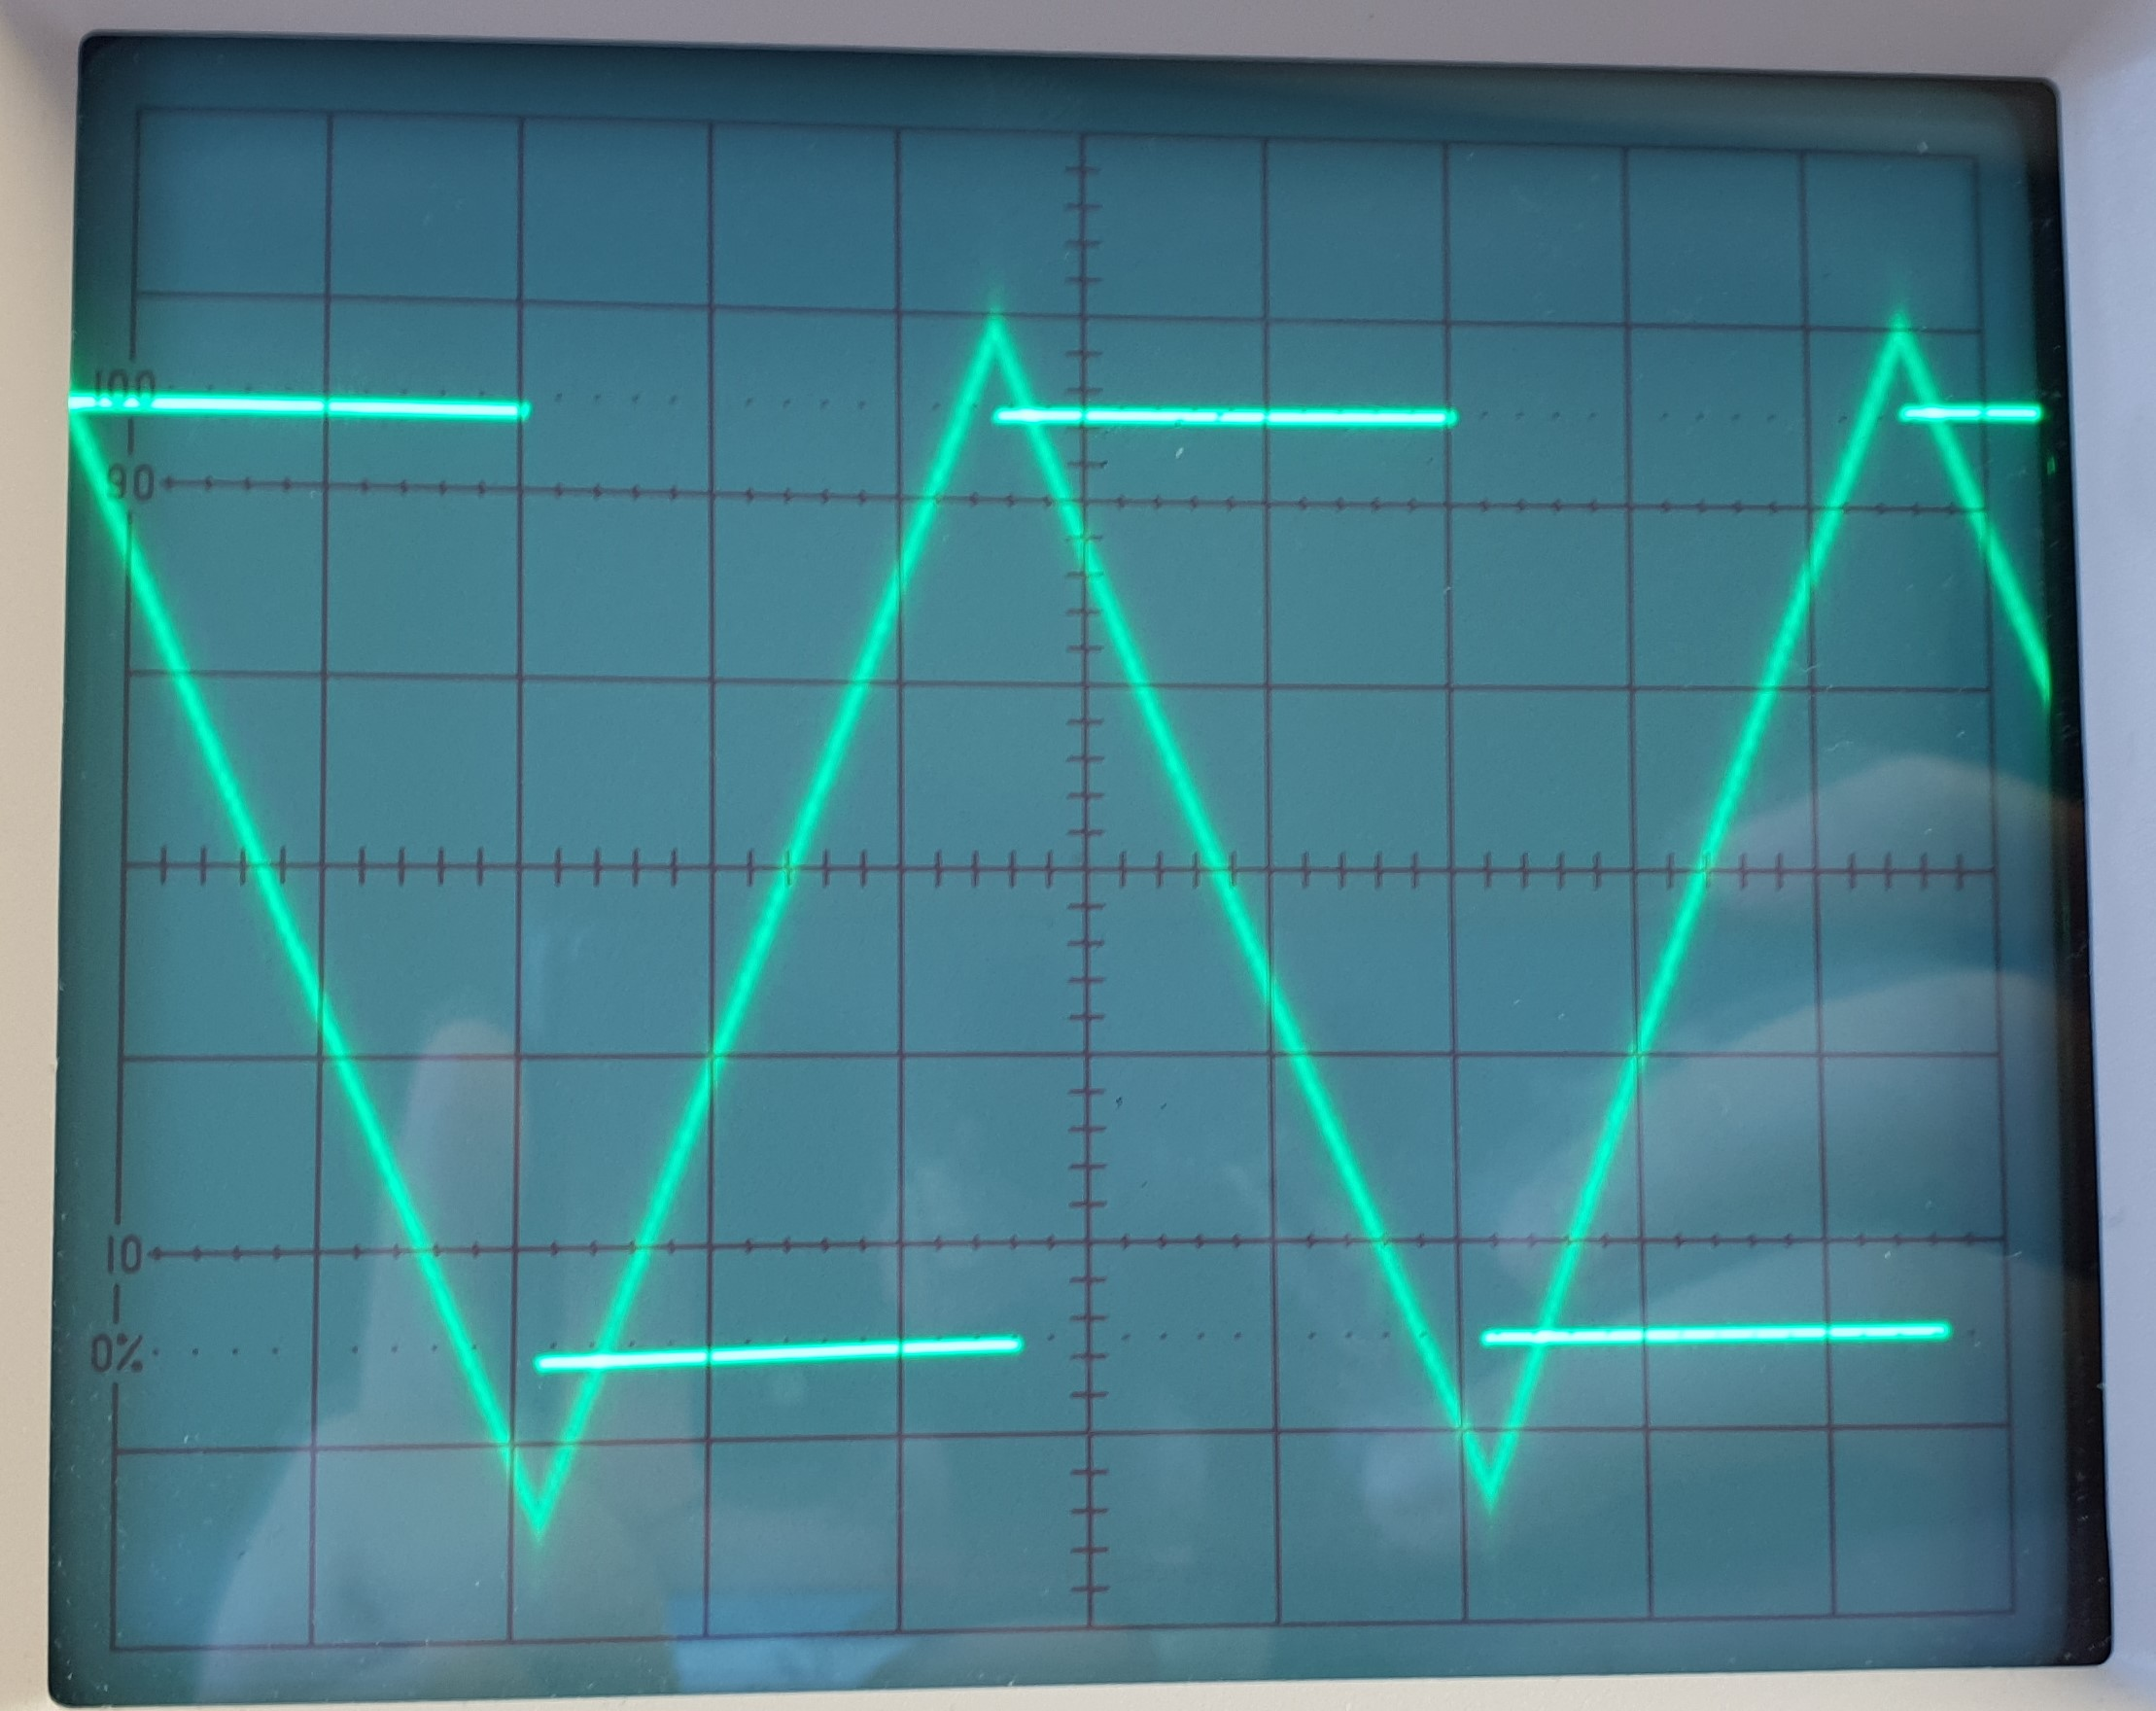
\includegraphics[width = \weite]{42-1000Hz.jpg}
    \end{tabular}
    \captionof{figure}{Umkehrintegrator bei zunehmender Frequenz}
    \label{abb:int}
\end{center}
Dabei ist zu bemerken, dass die entstehende Dreiecksspannung einen sichtbaren Phasenunterschied $\Delta\varphi$ vorweist. Das deckt sich mit der Erwartung der Integrationsschaltung, da die Ausgangsspannung $U_a$ der Eingangsspannung $U_e$ aufgrund des Kondensators $C_2$ bei höheren Frequenzen um $\Delta\varphi = \frac{\pi}{2}$ nachhinkt. Dieser Umstand lässt sich auch mit Gleichung (2.19) herleiten, wobei daraus folgt:
\begin{gather}
    \begin{aligned}
        U_a(t) &= - \frac{R_2}{R_1} \frac{1}{1+i\omega R_2 C_2} U_e(t)\\[0.5cm]
        \Leftrightarrow \frac{U_a}{U_e} &= v_{i,2} = - \frac{R_2}{R_1} \frac{1}{1+i\omega R_2 C_2} = - \frac{R_2}{R_1} \frac{1 - i\omega R_2 C_2}{1+(\omega R_2 C_2)^2}
    \end{aligned}\\[0.5cm]
    \Rightarrow \Delta\varphi = \arctan(\frac{\imaginary(v_{i,2})}{\real(v_{i,2})}) = \arctan(\omega R_2 C_2) \xrightarrow{\omega \rightarrow \infty} \frac{\pi}{2} 
\end{gather}
Betrachtet man nun die Gleichung \ref{eq:wi2} ergibt sich für diese Schaltung mit den Widerständen 
\begin{gather*}
    R_1 = (10.0 \pm 0.3)~\text{k}\Omega,~R_2 = (1.00 \pm 0.03)~\text{M}\Omega~\text{und}~C_2 = (10.0 \pm 0.3)~\text{nF},
\end{gather*}
wobei dabei der Fehler der Widerstände mit $3\%$ des Messwerts abgeschätzt und der Kondensator einen vom Hersteller angegebenen Fehler von $2.5\%$ des angegeben Wertes hat, für die Grenzfrequenz $f_{i,2}$ mit dem Fehler $s_{f_{i,2}}$ (ermittelt durch das Fehlerfortpflanzungsgesetz):
\begin{gather}
    f_{i,2} = \frac{1}{2\pi R_2 C_2} = 15.91549~\text{Hz}\\[0.5cm]
    s_{f_{i,2}} = \frac{1}{2\pi}\sqrt{\left(\frac{s_{R_2}}{R_2^2 C_2}\right)^2 + \left(\frac{s_{C_2}}{R_2 C_2^2}\right)^2} = 0.67523~\text{Hz}\\[0.5cm]
    \Rightarrow \boxed{f_{i,2} = (15.9 \pm 0.7)~\text{Hz}}
\end{gather}
Dieses Ergebnis deckt sich mit der Messung, da bei einer Frequenz von $100~\text{Hz}$ erkennt man in Abbildung \ref{abb:int} schon die Dreiecksspannung, währendessen bei einer Frequenz von $10~\text{Hz}$ das Signal der Ausgangsspannung $U_a$ die Ladekurve des Kondensators zeigt. Dies hat den Grund, dass der OPV ungefähr ab der Grenzfrequenz $f_{i,2}$ linear arbeitet und korrekt integriert. Weiterhin lässt sich durch Erhöhung der Frequenz der Spannungsquelle durch die Einstellungen am Oszilloskop (siehe S.22) gut erkennen, dass die Verstärkung frequenzabhängig ist.\\
 \\
Für den theoretischen Verlauf der Verstärkung $v_{i,2}$ betrachten wir Gleichung (2.20) mit $\omega = 2\pi f$.
%, woraus für dessen Fehler mit dem Fortpflanzungsgesetz folgt:
%\begin{gather}
%    s_{v_{i,2}} = v_{i,2} \sqrt{\left(\frac{s_{R_2}}{R_2(1+(\omega R_2C_2)^2)}\right)^2+\left(\frac{s_{R_1}}{R_1}\right)^2+\left(\frac{\omega^2 R_2^2 C_2 s_{C_2}}{1+(\omega R_2 C_2)^2}\right)^2}
%\end{gather}
Für den Fehler des Oszilloskop wird ein Ablesefehler $s_a = 0.1~\text{Div}$ und ein Restfehler $s_r = 0.03\cdot\text{Messwert in Div}$ verwendet, woraus mit der Einstellung des Oszilloskops folgt:
\begin{gather}
    U = \text{Messwert}\cdot\text{Einstellung} = [\text{Div}]\cdot[\text{V/Div}]\\
    s_U = [\text{V/Div}]\sqrt{(0.03\cdot [\text{Div}])^2 + (0.1~[\text{Div}])^2} 
\end{gather}
Daraus folgt auch der Fehler für die Verstärkung $v$ mit dem Fehlerfortpflanzungsgesetz wie folgt:
\begin{gather}
    v = \frac{U_a}{U_a} \Rightarrow s_v = \sqrt{\left(\frac{s_{U_a}}{U_e}\right)^2 + \left(\frac{U_a s_{U_e}}{(U_e)^2}\right)^2}
\end{gather}
Mit einsetzen der Messwerte folgt dann folgende Tabelle \ref{tab:int}, wobei der Messwert 1 ausgesondert wird, da dieser nicht korrekt ablesbar war und ab Messwert 19 ein Ablesefehler $s_a = 0.5~\text{Div}$ verwendet wird, da diese Werte bei der Messung sehr schwer abzulesen waren.
\newpage
\begin{center}
    \captionof{table}{Messreihe Umkehrintegrator}
    \begin{tabular}{l c c c c c | c c}
        {} &   $f$/Hz &  $U_a$/V &  $s_{U_a}$/V &  $U_e$/V &  $s_{U_e}$/V 
        &      $v$ &   $s_v$ \\
        \hline
        1  &      5 &  4.000 &      0.156 &   0.050 &      0.002 &  80.00 &  4.25 \\
        2  &     10 &  4.000 &      0.156 &   0.050 &      0.002 &  80.00 &  4.25 \\
        3  &     14 &  3.800 &      0.152 &   0.050 &      0.002 &  76.00 &  4.09 \\
        4  &     17 &  3.500 &      0.145 &   0.050 &      0.002 &  70.00 &  3.84 \\
        5  &     21 &  3.000 &      0.135 &   0.050 &      0.002 &  60.00 &  3.45 \\
        6  &     28 &  2.500 &      0.090 &   0.050 &      0.002 &  50.00 &  2.55 \\
        7  &     37 &  2.000 &      0.078 &   0.050 &      0.002 &  40.00 &  2.13 \\
        8  &     52 &  1.500 &      0.067 &   0.050 &      0.002 &  30.00 &  1.73 \\
        9  &     56 &  1.400 &      0.047 &   0.050 &      0.002 &  28.00 &  1.37 \\
        10 &     66 &  1.200 &      0.041 &   0.050 &      0.002 &  24.00 &  1.19 \\
        11 &     78 &  1.000 &      0.036 &   0.050 &      0.002 &  20.00 &  1.02 \\
        12 &    100 &  0.800 &      0.031 &   0.050 &      0.002 &  16.00 &  0.85 \\
        13 &    110 &  0.700 &      0.023 &   0.050 &      0.002 &  14.00 &  0.69 \\
        14 &    130 &  0.600 &      0.021 &   0.050 &      0.002 &  12.00 &  0.60 \\
        15 &    160 &  0.500 &      0.018 &   0.050 &      0.002 &  10.00 &  0.51 \\
        16 &    210 &  0.400 &      0.016 &   0.050 &      0.002 &   8.00 &  0.43 \\
        17 &    280 &  0.300 &      0.013 &   0.050 &      0.002 &   6.00 &  0.35 \\
        18 &    440 &  0.200 &      0.050 &   0.050 &      0.002 &   4.00 &  1.02 \\
        19 &    800 &  0.100 &      0.025 &   0.050 &      0.002 &   2.00 &  0.51 \\
        20 &   2100 &  0.040 &      0.005 &   0.050 &      0.002 &   0.80 &  0.11 \\
        21 &   3100 &  0.030 &      0.005 &   0.050 &      0.002 &   0.60 &  0.10 \\
        22 &   5800 &  0.020 &      0.005 &   0.050 &      0.002 &   0.40 &  0.10 \\
        23 &   7500 &  0.015 &      0.003 &   0.050 &      0.002 &   0.30 &  0.05 \\
        24 &  10000 &  0.012 &      0.003 &   0.050 &      0.002 &   0.24 &  0.05 \\
    \end{tabular}
    \label{tab:int}
\end{center}
Trägt man die Verstärkung $v$ doppellogarithmisch gegen die Frequenz $f$ auf erhält man Abbildung \ref{abb:intMess}. Dabei ist deutlich zu erkennen, dass die Messung in Rahmen der Messgenauigkeit gut getroffen wurde. Auch ist die Grenzfrequenz $f_{i,2}$ durch die Messung nochmal bestätigt und es lässt sich gut der lineare Bereich des OPVs erkennen, indem dieser korrekt integriert.
\newpage
\begin{center}
    \captionof{figure}{Frequenzgang des Umkehrintegrator}
    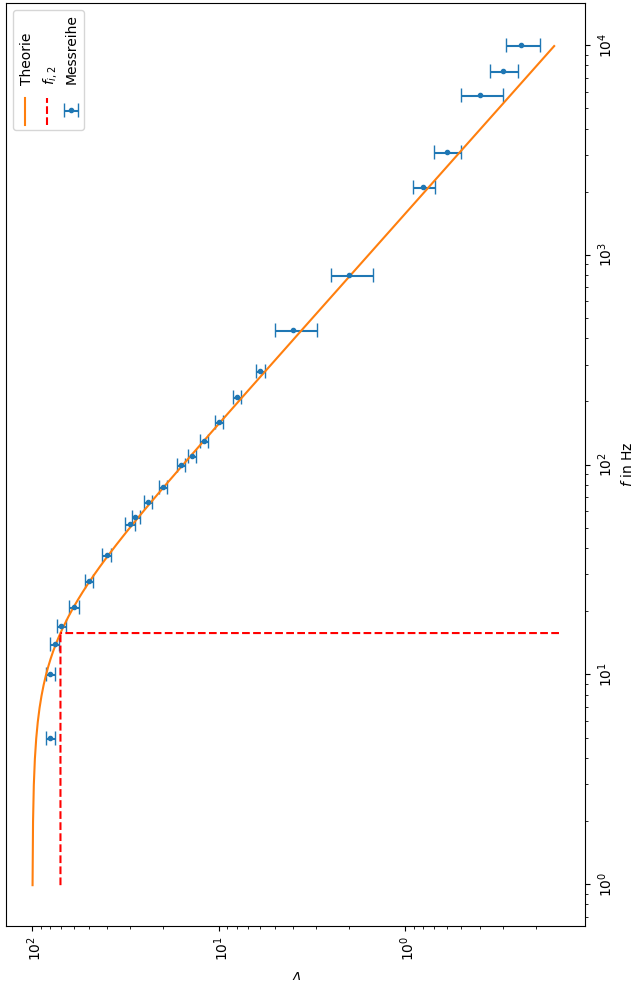
\includegraphics[scale = 0.75]{intOPVlogMess.png}
    \label{abb:intMess}
\end{center}
